
\documentclass[10pt,conference]{IEEEtran}
\usepackage[utf8]{inputenc}
\usepackage[T1]{fontenc}
\usepackage{amsmath,amssymb}
\usepackage{graphicx}
\usepackage{booktabs}
\usepackage{multirow}
\usepackage{array}
\usepackage{url}
\usepackage[hidelinks]{hyperref}
\setlength{\textfloatsep}{4pt plus 1pt minus 1pt}
\setlength{\floatsep}{4pt plus 1pt minus 1pt}
\setlength{\intextsep}{5pt plus 1pt minus 1pt}
\setlength{\abovecaptionskip}{3pt}
\setlength{\belowcaptionskip}{0pt}
\renewcommand{\arraystretch}{0.94}
\setlength{\parskip}{0pt}
\hyphenpenalty=1000
\sloppy
\begin{document}
\title{\vspace{-1.2em}\normalsize THE UNIVERSITY OF LAHORE $\bullet$ DEPARTMENT OF INTELLIGENT SYSTEMS $\bullet$ AI-101\\[2pt]
\Large Task A1: Breast Cancer Diagnosis from Cell-Nucleus Measurements}
\author{\normalsize Rizwan Ali \quad|\quad Roll No.\ 70177926 \quad|\quad Section C\\
\normalsize\url{https://github.com/RaeesRizwan09/AI101-ML-Assignment-70177926} \quad|\quad Instructor: Dr.\ Muhammad Awais, AI Architect}
\maketitle
\vspace{-1.4em}
\begin{center}\small\itshape A logistic regression reaches ROC-AUC 0.996 and catches 39/42 malignancies at the default threshold, while a majority-class model is 0.632 accurate and catches none.\end{center}
\vspace{-0.6em}

\section{Introduction}
Fine-needle aspiration (FNA) is the least invasive way to sample a suspicious breast
mass: a thin needle lifts a few cells and software measures the nuclei. Measurements are
cheap but their reading is subjective, so a model mapping them to a malignancy probability
can act as a \emph{second reader} that flags ambiguous cases. What makes the problem
interesting is not accuracy but the \emph{cost asymmetry}: a false negative
delays cancer treatment, whereas a false positive costs one unnecessary biopsy. A
screening model must therefore be evaluated at a high-recall operating point, and accuracy
-- dominated by the 62.74\% benign majority -- is close to
meaningless. I trained and tuned five models under one leakage-free protocol and find that
a scaled logistic regression matches non-linear alternatives, that the 95\% recall
constraint is already satisfied at the default threshold, and that 7 of the
30 features are redundant at no measurable cost.

\section{Problem Statement}
Each sample is $x\in\mathbb{R}^{30}$: ten nucleus properties (radius, texture,
perimeter, area, smoothness, compactness, concavity, concave points, symmetry, fractal
dimension), each summarised as mean, standard error and worst value; the label is
$y\in\{\text{malignant},\text{benign}\}$. We learn
$f:\mathbb{R}^{30}\to[0,1]$ approximating $P(y=\text{malignant}\mid x)$ and predict
malignant iff $f(x)\ge\tau$. This is supervised binary classification, scored by recall and
F1 on the malignant class and by ROC-AUC, under the constraint that missed malignancies
cost far more than false alarms. The data are mildly imbalanced
(212/357) and come from a single
institution, which bounds external validity.

\section{Dataset Used}
Breast Cancer Wisconsin (Diagnostic), UCI ML Repository id~17~\cite{uci}, also
distributed with scikit-learn~\cite{sklearn}. Street, Wolberg and Mangasarian collected
it in 1993 from digitised FNA images at the University of Wisconsin Hospitals and released
it for research use. Each of the 569 rows is one patient's sample, the
30 columns are the ten properties in three summaries, and the target is the
cytological diagnosis. The shipped encoding is $0=$malignant, $1=$benign, so I flipped it
immediately to make \emph{malignant $=1=$ positive} and audited every metric against that
convention -- inverting it would silently invert the entire report. No rows were removed:
0.0\% of cells are missing and there are no duplicates.

\section{Dataset Statistics}
Table~\ref{tab:stats} summarises the data and Figure~\ref{fig:eda} the class balance.
The minority class (212 samples) is large enough that
stratification, not resampling, is the right response. The correlation matrix (notebook
Fig.~2) has the expected block structure -- radius, perimeter and area move together
($r>0.99$), as do concavity and concave points -- so a union-find over all pairs with
$|r|\ge0.95$ \emph{on the training split only} yields 2 groups
covering 7 droppable features.


\begin{table}[t]
\centering
\caption{Dataset statistics (no rows removed).}
\label{tab:stats}
\scriptsize
\begin{tabular}{l@{\hspace{2pt}}l@{\hspace{6pt}}l@{\hspace{2pt}}l}
\toprule
Property & Value & Property & Value \\
\midrule
Samples & 569 & Features & 30 numeric \\
Missing values & 0.0\% & Train / test & 455 / 114 \\
Malignant & 212 (37.26\%) & Benign & 357 (62.74\%) \\
\bottomrule
\end{tabular}
\end{table}



\begin{figure}[t]
\centering
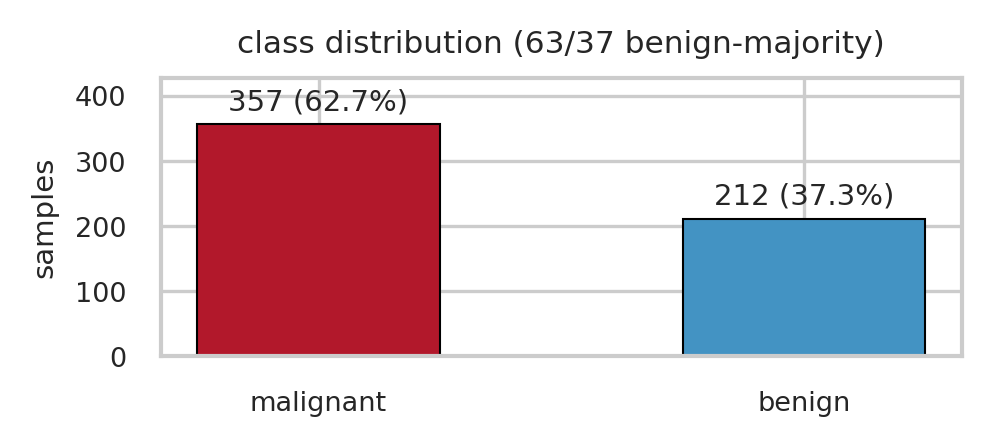
\includegraphics[width=\columnwidth]{figures/A1_fig1_class_distribution.png}
\caption{EDA: class balance. The benign majority is what makes accuracy misleading; mean nucleus radius separates the classes but overlaps in the 12--16\,$\mu$m band where the errors live (notebook Fig.~1b).}
\label{fig:eda}
\end{figure}


\section{Methodology}
\subsection{Learning setting}
Supervised binary classification on a small ($n=569$), low-dimensional
($d=30$), strongly collinear tabular dataset. I compared a majority-class
\emph{Dummy} model (a diagnostic that quantifies the accuracy trap), a \emph{Logistic
Regression} baseline, an \emph{RBF SVM} (non-linear, strong at this sample size),
\emph{k-NN} ($k=5$, untuned, as an instance-based reference) and a \emph{Random Forest}
(gives importances). All scaling lives inside a \texttt{Pipeline}, fitted on training
folds only.

\subsection{Data-split approach}
One stratified 80/20 split (\texttt{random\_state=42}) gives
455/114 samples with the class ratio preserved. Hyperparameters are
chosen by \texttt{GridSearchCV} with 5-fold \texttt{StratifiedKFold} on the training
split only, selecting on ROC-AUC; the test set is scored once. Two subtler leakage routes
are closed explicitly: the redundancy analysis uses the training correlation matrix, and
the threshold is chosen on \emph{out-of-fold} training predictions, never on test labels.

\subsection{Parameter settings}

\begin{table}[t]
\centering
\caption{Hyperparameter spaces and selected values (selection metric: CV ROC-AUC).}
\label{tab:hp}
\scriptsize
\begin{tabular}{p{1.45cm}p{2.5cm}p{1.55cm}}
\toprule
Model & Search space (5-fold CV) & Selected \\
\midrule
Logistic Reg. & $C\in\{10^{-3}\!\dots\!10^{2}\}$, L2 & $C=1$ \\
SVM (RBF) & $C\in\{.1,1,10,100\}$, $\gamma\in\{\mathrm{sc},.01,.1\}$ & $C=10$, $\gamma=0.01$ \\
Rand.\ Forest & trees $\in\{200,400\}$, depth $\in\{-,4,6,8\}$, leaf $\in\{1,2,4\}$ & 200, d$=8$ \\
k-NN & untuned & $k=5$ \\
\bottomrule
\end{tabular}
\end{table}


\section{Results and Analysis}
\subsection{Results}
Table~\ref{tab:res} is the single test evaluation. The model ranking is decided by
cross-validation, not by the test column: LogisticRegression has the highest CV ROC-AUC
(0.996 $\pm$ 0.005), with the SVM statistically
indistinguishable (0.995 $\pm$
0.005). The Dummy row is the point of the exercise.


\begin{table}[t]
\centering
\caption{Test-set results (n=114), scored once after tuning; malignant = positive. Best per column in bold. 5-fold CV ROC-AUC on the training split (mean$\pm$sd): LR 0.996\(\pm\)0.005, SVM 0.995\(\pm\)0.005, RF 0.989\(\pm\)0.007.}
\label{tab:res}
\scriptsize
\begin{tabular}{lccccc}
\toprule
Model & Acc. & Prec. & Rec. & F1 & ROC-AUC \\
\midrule
DummyMajority & 0.632 & 0.000 & 0.000 & 0.000 & 0.500 \\
kNN k5 & 0.956 & 0.974 & 0.905 & 0.938 & 0.982 \\
LogisticRegression & 0.965 & 0.975 & 0.929 & 0.951 & \textbf{0.996} \\
SVM RBF & \textbf{0.982} & \textbf{1.000} & \textbf{0.952} & \textbf{0.976} & \textbf{0.996} \\
RandomForest & 0.965 & \textbf{1.000} & 0.905 & 0.950 & 0.994 \\
\bottomrule
\end{tabular}
\end{table}



\begin{figure}[t]
\centering
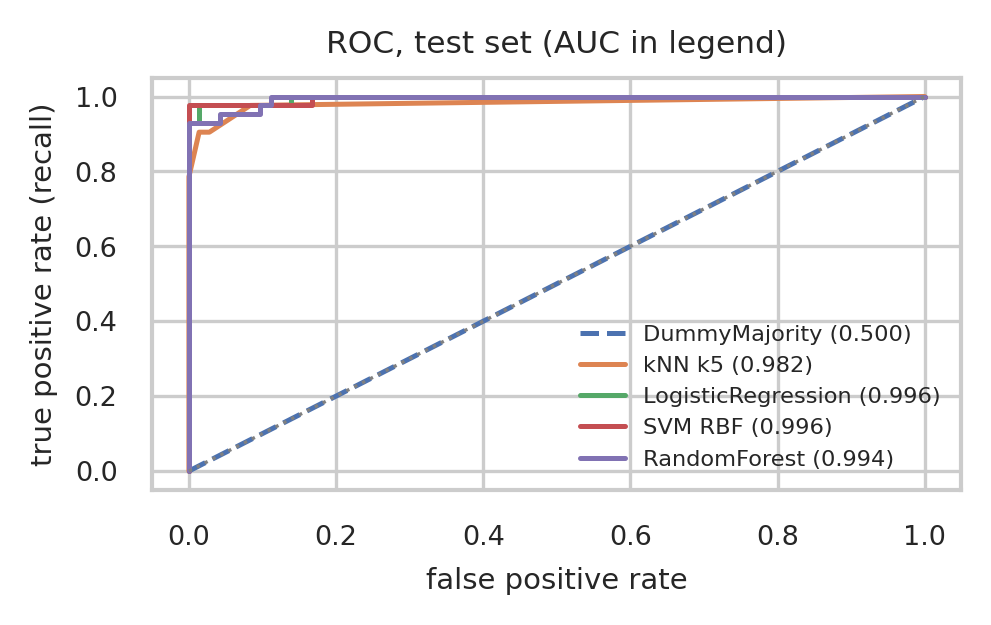
\includegraphics[width=\columnwidth]{figures/A1_fig4_roc.png}
\caption{ROC curves on the test set. The Dummy model is the diagonal; the four real models are nearly coincident above 0.98.}
\label{fig:roc}
\end{figure}



\begin{figure}[t]
\centering
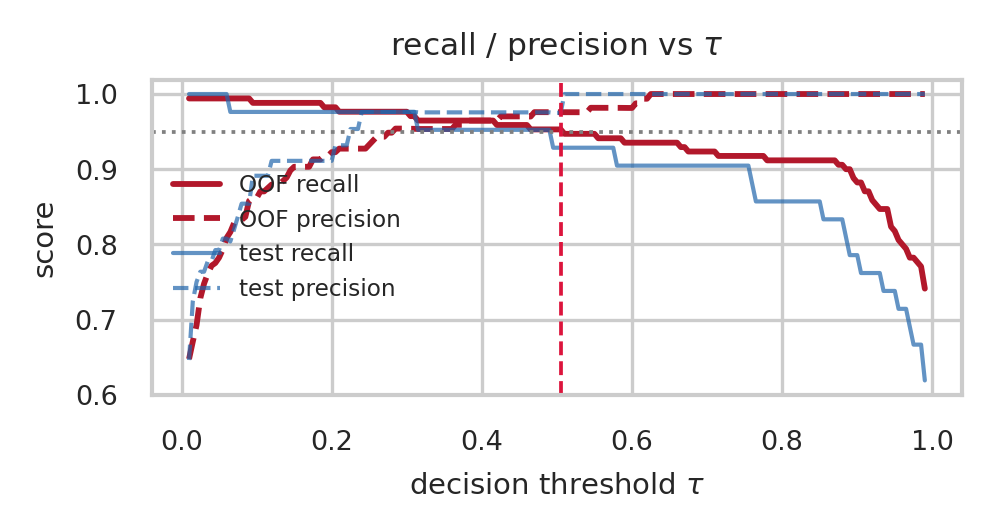
\includegraphics[width=\columnwidth]{figures/A1_fig6_threshold.png}
\caption{Threshold study. $\tau^*$ is chosen on out-of-fold training predictions (red) and then applied once to the test set (blue, descriptive only).}
\label{fig:thr}
\end{figure}


\subsection{Analysis}
\textbf{Which model, and why accuracy misleads.} The majority-class model is
0.632 accurate with recall 0.000: it calls every
patient benign and therefore misses all 42 cancers in the test set. Accuracy rewards
it for the 62.74\% prior, which is why selection here uses ROC-AUC
(ranking) plus malignant recall and F1 (operating point). Among real models differences are
small: after standardisation the classes are nearly linearly separable along a size
direction, so the linear baseline already reaches 0.996 AUC and the
non-linear models buy at most 0.000 AUC.
With 569 samples, the split and the threshold matter more than the model class.

\textbf{What the threshold buys.} At
$\tau=0.50$ the model already achieves recall 0.929 at precision
0.975, so the 95\% constraint is met without moving the threshold and
$\tau^*=0.505$ (the largest threshold still satisfying it) costs
0.0 precision points -- essentially
nothing. The mechanism only becomes visible when the constraint is tightened: demanding
99\% recall pushes $\tau$ to 0.090, converts 2 false negatives
into true positives, and costs 6 extra false positives and
12.1 precision points. That exchange rate is
what a clinic negotiates, and it is invisible in a single accuracy number. Note that a
naive test-set sweep would have picked $\tau=0.49$ and reported a recall gain partly fitted
to the test labels.

\textbf{Features and redundancy.} The Random Forest ranks worst perimeter, worst area, worst concave points first, and the
logistic coefficients agree in sign: larger, more concave, more irregular nuclei imply
malignancy. Dropping one feature from every $|r|\ge0.95$ group (23 of 30 remain) changes test AUC by
-0.0010 (to 0.9950) and F1 by +0.0117
(to 0.9630): the redundant
features carry no information the survivors do not, and L2 regularisation already absorbs
their collinearity; recall does move from 0.929 to
0.929, which is one test case and well inside 114-sample noise.
They still matter for \emph{interpretation} -- reporting radius, perimeter and area as
three separate risk factors triple-counts one geometric property.

\textbf{Errors and limitations.} At $\tau^*$ there are 4 test
errors: 3 false negative (a 13.8\,$\mu$m, low-concavity malignant sample
inside the benign cloud) and 1 false positive (a benign sample with
above-average concavity) -- genuine distributional overlap, not a coding fault.
Limitations: one institution and scanner, no external validation, and $\tau^*$ estimated
from a small out-of-fold set.

\section{Conclusion}
A scaled logistic regression matches non-linear alternatives here (ROC-AUC
0.996, 39/42 malignancies caught at $\tau=0.50$), and the
95\% recall constraint is free because the classes are nearly separable; tuning SVM and
forest bought a fraction of an AUC point. Next I would validate externally and replace the
hard threshold with a calibrated risk score.

\section*{AI Use Disclosure}
I used Claude (Anthropic) as an AI assistant for scaffolding this notebook, writing plotting
boilerplate, and drafting report prose from the numbers the notebook produced. The
following parts were generated or substantially assisted by AI: the notebook's cell
structure and plotting code, and the first draft of Sections I--VII. I verified this
content by re-running every cell end to end, checking metrics against the scikit-learn
documentation and the course slides, and recomputing the headline numbers by hand from the
saved CSVs. I also corrected two methodological errors in the AI's first draft: the
positive-class encoding and the use of the test set to choose the decision threshold. All
experiments, results and analysis in this report were produced and checked by me, and I
take full responsibility for this work.

\begin{thebibliography}{9}
\bibitem{uci} W.~N. Street, W.~H. Wolberg, and O.~L. Mangasarian, ``Nuclear feature
extraction for breast tumor diagnosis,'' in \emph{Proc.\ IS\&T/SPIE Symp.\ Electronic
Imaging}, 1993. UCI ML Rep.\ id~17.
\bibitem{sklearn} F.~Pedregosa \emph{et al.}, ``Scikit-learn: Machine learning in
Python,'' \emph{JMLR}, vol.~12, pp.~2825--2830, 2011.
\bibitem{fawcett} T.~Fawcett, ``An introduction to ROC analysis,'' \emph{Pattern
Recognition Letters}, vol.~27, no.~8, pp.~861--874, 2006.
\end{thebibliography}
\end{document}
